\documentclass[11pt]{article}

\usepackage[letterpaper,margin=0.88in,headheight=22pt]{geometry}
\usepackage{fontspec}
\IfFontExistsTF{Charis SIL}{\setmainfont{Charis SIL}}{\setmainfont{TeX Gyre Pagella}}
\IfFontExistsTF{Arimo}{\setsansfont{Arimo}}{\setsansfont{TeX Gyre Heros}}
\usepackage{microtype}
\usepackage{amsmath,amssymb}
\usepackage{siunitx}
\usepackage{booktabs}
\usepackage{tabularx}
\usepackage{longtable}
\usepackage{array}
\usepackage{enumitem}
\usepackage{xcolor}
\usepackage{colortbl}
\usepackage{graphicx}
\usepackage{tikz}
\usetikzlibrary{arrows.meta,positioning,calc,decorations.pathreplacing}
\usepackage[most]{tcolorbox}
\usepackage{titlesec}
\usepackage{fancyhdr}
\usepackage{caption}
\usepackage{float}
\usepackage[hidelinks]{hyperref}
\usepackage{lastpage}
\usepackage{needspace}
\usepackage{graphbox} % Extends graphicx

% University of Texas at Austin brand palette
\definecolor{UTBurntOrange}{HTML}{BF5700}
\definecolor{UTCharcoal}{HTML}{333F48}
\definecolor{UTLightOrange}{HTML}{F8971F}
\definecolor{UTWarmGray}{HTML}{D6D2C4}
\definecolor{UTSlate}{HTML}{9CADB7}
\definecolor{UTBlue}{HTML}{005F86}
\definecolor{UTBlueBright}{HTML}{00A9B7}
\definecolor{UTWarmLight}{HTML}{F6F5F2}
\definecolor{UTBlueLight}{HTML}{EEF5F7}
\definecolor{UTGrayLight}{HTML}{F4F5F6}

% Backward-compatible semantic aliases used throughout the document
\colorlet{Navy}{UTCharcoal}
\colorlet{Teal}{UTBurntOrange}
\colorlet{LightTeal}{UTBlueLight}
\colorlet{LightBlue}{UTWarmLight}
\colorlet{LightGray}{UTGrayLight}
\colorlet{MidGray}{UTCharcoal!78}
\colorlet{RuleGray}{UTWarmGray}
\colorlet{Warn}{UTLightOrange}
\colorlet{LightWarn}{UTWarmLight}

\hypersetup{
  colorlinks=true,
  linkcolor=UTBurntOrange,
  urlcolor=UTBlue,
  citecolor=UTCharcoal,
  pdftitle={STNCL Phase-Specific Experimental Plan},
  pdfauthor={TRIDENT Collaboration (UT Austin, ACU, VCU)}
}

\sisetup{
  detect-all,
  per-mode=symbol,
  range-phrase=--,
  range-units=single,
  group-separator={,},
  group-minimum-digits=4,
  group-digits=integer
}

\setlength{\parindent}{0pt}
\setlength{\parskip}{5.5pt}
\setlength{\emergencystretch}{1.5em}
\setlist[itemize]{leftmargin=1.35em,itemsep=2.5pt,topsep=3pt}
\setlist[enumerate]{leftmargin=1.55em,itemsep=3pt,topsep=3pt}
\renewcommand{\arraystretch}{1.18}
\titlespacing{\paragraph}{0pt}{0.5ex plus 0.5ex minus .2ex}{1em}

\titleformat{\section}
  {\Large\sffamily\bfseries\color{UTBurntOrange}}
  {\thesection}{0.65em}{}
  [\vspace{1pt}\color{UTWarmGray}\titlerule]
\titleformat{\subsection}
  {\large\sffamily\bfseries\color{UTCharcoal}}
  {\thesubsection}{0.6em}{}
\titleformat{\subsubsection}
  {\normalsize\sffamily\bfseries\color{UTCharcoal}}
  {\thesubsubsection}{0.55em}{}
\titlespacing*{\section}{0pt}{14pt}{7pt}
\titlespacing*{\subsection}{0pt}{11pt}{4pt}
\titlespacing*{\subsubsection}{0pt}{8pt}{2pt}

% Keep a heading from being stranded alone at the bottom of a page:
% require room for the title plus a few body lines, else break to the next page.
\usepackage{etoolbox}
\pretocmd{\section}{\needspace{5\baselineskip}}{}{}
\pretocmd{\subsection}{\needspace{7\baselineskip}}{}{}
\pretocmd{\subsubsection}{\needspace{5\baselineskip}}{}{}

\pagestyle{fancy}
\fancyhf{}
\fancyhead[L]{\small\sffamily\color{UTCharcoal}Prop-30 Glycol STNCL \textbullet\ TRIDENT}
\fancyhead[R]{\small\sffamily\color{UTBurntOrange}\PhaseDocShort -- Draft}
\fancyfoot[L]{\small\sffamily\color{UTCharcoal!78}Revision 0.1}
\fancyfoot[R]{\small\sffamily\color{UTCharcoal!78}Page \thepage\ of \pageref{LastPage}}
\renewcommand{\headrulewidth}{0.65pt}
\renewcommand{\headrule}{\hbox to\headwidth{\color{UTBurntOrange}\leaders\hrule height \headrulewidth\hfill}}
\renewcommand{\footrulewidth}{0pt}

\newtcolorbox{recommendbox}[1][]{
  enhanced,
  breakable,
  colback=UTWarmLight,
  colframe=UTBurntOrange,
  colbacktitle=UTBurntOrange,
  boxrule=0.7pt,
  arc=1.2mm,
  left=3mm,right=3mm,top=2.4mm,bottom=2.4mm,
  title={#1},
  fonttitle=\sffamily\bfseries,
  coltitle=white
}

\newcommand{\Tavg}{T_{\mathrm{avg},4}}
\newcommand{\Tdiag}{T_{\mathrm{diag}}}
\newcommand{\Thot}{T_{\mathrm{hot}}}
\newcommand{\Tcold}{T_{\mathrm{cold}}}
\newcommand{\QHs}{\dot Q_{H}^{s}}
\newcommand{\QCs}{\dot Q_{C}^{s}}
\newcommand{\mdotp}{\dot m_{p}}
\newcommand{\mdotpH}{\dot m_{p,H}}
\newcommand{\mdotpC}{\dot m_{p,C}}
\newcommand{\Tamb}{T_{\mathrm{amb}}}
\newcommand{\Rey}{\mathrm{Re}}
\newcommand{\Realpart}[1]{\Re\left(#1\right)}

\newcommand{\PhaseDocShort}{Phase 1: Ambient-Equilibrium Baseline}

% Cross-document names used instead of duplicating material owned by another phase.
\newcommand{\PhaseZeroDoc}{\textit{Phase 0 --- System Checkout}}
\newcommand{\PhaseOneDoc}{\textit{Phase 1 --- Ambient-Equilibrium Baseline}}
\newcommand{\PhaseTwoDoc}{\textit{Phase 2 --- Thermal Relaxation Tests}}
\newcommand{\PhaseThreeDoc}{\textit{Phase 3 --- Low-Duty Steady Heat-Loss Tests}}
\newcommand{\PhaseFourDoc}{\textit{Phase 4 --- Initial Test Matrix and Transition Characterization}}

\begin{document}
\hypersetup{pageanchor=false}

\begin{titlepage}
\thispagestyle{empty}
\begin{tikzpicture}[remember picture,overlay]
  \fill[UTBurntOrange] (current page.north west) rectangle ([yshift=-0.16in]current page.north east);
  \fill[UTWarmLight] ([yshift=1.45in]current page.south west) rectangle (current page.south east);
  \fill[UTBurntOrange] (current page.south west) rectangle ([yshift=0.16in]current page.south east);
\end{tikzpicture}
\noindent
\includegraphics[width=2.5in]{images/TRIDENT_logo.png}

{\color{UTWarmGray}\rule{\textwidth}{0.8pt}}
\vspace{0.24in}
\begin{tcolorbox}[
  enhanced, frame hidden, colback=white, boxrule=0pt,
  borderline west={4pt}{0pt}{UTBurntOrange},
  left=5mm,right=0mm,top=1mm,bottom=1mm, sharp corners
]
{\raggedright\sffamily\bfseries\fontsize{23}{27}\selectfont\color{UTCharcoal}
Experimental Plan for the Initial Characterization of the Prop-30 Glycol Salt Twin Natural Circulation Loop (STNCL)\par}
\vspace{0.15in}
{\sffamily\bfseries\fontsize{16}{20}\selectfont\color{UTBurntOrange}
Phase 1: Ambient-Equilibrium Baseline\par}
\vspace{0.10in}
{\sffamily\fontsize{11.5}{15}\selectfont\color{UTCharcoal}
Installed measurement performance, uncertainty resolution, and acceptance-method calibration\par}
\end{tcolorbox}

\vspace{0.30in}
\begin{tcolorbox}[
  enhanced, colback=UTWarmLight, colframe=UTWarmGray, boxrule=0.6pt,
  arc=1.2mm, left=3.5mm,right=3.5mm,top=3mm,bottom=3mm
]
{\setlength{\parskip}{0pt}\renewcommand{\arraystretch}{1.28}
\begin{tabularx}{\textwidth}{@{}>{\sffamily\bfseries\color{UTBurntOrange}}l>{\raggedright\arraybackslash}X@{}}
Status: & Draft for team review and facility-specific completion \\
Revision: & 0.1 \\
Date: & August 17, 2026 \\
Prepared for: & TRIDENT collaboration \\
\end{tabularx}}
\end{tcolorbox}

\vfill
\noindent

\includegraphics[height=2.5cm, align=c]{images/ACU.png}\hfill

\includegraphics[height=1.5cm, align=c]{images/UT.png}\hfill

\includegraphics[height=1.25cm, align=c]{images/VCU.png}
\vspace{-0.6in}
\end{titlepage}
\clearpage
\hypersetup{pageanchor=true}

\clearpage
\pagenumbering{roman}
\section*{Revision History}
\addcontentsline{toc}{section}{Revision History}
\begin{tabularx}{\textwidth}{@{}p{0.75in}p{1.2in}>{\raggedright\arraybackslash}X>{\raggedright\arraybackslash}p{1.15in}@{}}
\toprule
\textbf{Revision} & \textbf{Date} & \textbf{Description} & \textbf{Status} \\
\midrule
0.1 & 2026-08-17 & Phase-specific split of the initial characterization plan; technical content retained with cross-document references where material is owned by an earlier phase. & Draft \\
\bottomrule
\end{tabularx}

\vspace{0.25in}
\section*{Approval and Configuration Record}
\addcontentsline{toc}{section}{Approval and Configuration Record}
\begin{tabularx}{\textwidth}{@{}p{1.55in}X p{1.25in}p{1.05in}@{}}
\toprule
\textbf{Role} & \textbf{Signature} & \textbf{Date} & \textbf{Revision} \\
\midrule
Lead, UT & & & \\
Lead, VCU & & & \\
Lead, ACU & & & \\
\bottomrule
\end{tabularx}
\clearpage
\tableofcontents
\clearpage
\pagenumbering{arabic}

\section{Introduction}
\label{sec:introduction}
\subsection{Purpose}
Phase~1 characterizes the installed measurement system with the filled loop near room temperature. The baseline is used to quantify noise, drift, autocorrelation, spatial consistency, TC--Luna agreement, room gradients, and the measurement resolution available for later near-isothermal and steady-state tests. It is not a verified zero-flow condition.

\subsection{Prerequisites and required data}
Phase~0 shall be dispositioned as \textbf{Proceed}. Use the approved Phase~0 configuration identifier, channel and geometry maps, acceptance-channel matrix and alternates, calibration and Type~B uncertainty information, synchronization verification, property references, environmental instrumentation, and operating limits. Apparatus geometry, station numbering, primary-temperature definitions, secondary-duty definitions, and the ambient heat-transfer sign convention are defined in \PhaseZeroDoc~and are not repeated here.

Phase~1 requires a filled loop in the approved passive configuration and a continuous synchronized ambient-equilibrium record long enough to characterize the relevant environmental cycle. Section~2 defines the statistical and uncertainty basis that Phase~1 must calibrate and freeze for use by the later phase documents.

\clearpage
\section{Technical Basis}
\label{sec:technical_basis}
\subsection{Data Acceptance and Uncertainty}
\label{sec:uncertainty}

\subsubsection{From a reporting requirement to an acceptance limit}

Acceptance limits shall be derived from the intended use of the data, not selected after a run to make it pass. Measurement uncertainty shall be evaluated using a documented measurement model consistent with the principles of JCGM~100 \cite{jcgm100}. For a reported result $y=f(x_1,\ldots,x_n)$, the combined standard uncertainty is
\begin{equation}
    u_y^2
    =
    \mathbf J\boldsymbol\Sigma_x\mathbf J^{\mathsf T},
    \qquad
    \mathbf J
    =
    \begin{bmatrix}
        \partial f/\partial x_1 & \cdots & \partial f/\partial x_n
    \end{bmatrix},
    \label{eq:propagation_matrix}
\end{equation}
where the sensitivity vector is evaluated at the reported input estimates and $\boldsymbol\Sigma_x$ contains their variances and covariances. Covariance is retained because common calibration, acquisition, property, or environmental errors may cancel in a difference or reinforce one another; assuming zero covariance is itself an assumption that shall be documented.

The covariance matrix combines three kinds of information. Type~A contributions are estimated from the accepted time series. The data are detrended only for estimating their correlation structure, divided into blocks longer than the relevant autocorrelation time, and reduced using the covariance of the block means so that densely sampled but correlated data are not treated as independent. The Phase~1 baseline (Section~\ref{sec:baseline}) supplies the initial block duration and correlation estimates, which shall be checked at later operating conditions. Type~B contributions represent shared calibration, DAQ, geometry, fluid-property, and other systematic sources that a single run cannot reveal. Thermal-model and repeatability contributions are added explicitly rather than hidden in the measurement covariance.

For this campaign, each limit is established by the same three-step chain:
\begin{enumerate}
    \item \textbf{Specify the reporting target.} Define the allowable uncertainty and its statistical meaning for the quantity to be reported, such as regional heat loss, corrected duty, inferred primary flow, or Reynolds number.
    \item \textbf{Allocate uncertainty and state-representativeness limits.} Allocate the uncertainty target among measurement, property, geometry, thermal-model, and repeatability effects and propagate those contributions through the measurement model. Separately allocate acceptable spatial and temporal variation so that one reported value adequately represents the accepted interval. For an approximately linear signal with fitted slope $b$, the interval mean equals the value at the temporal midpoint, while either endpoint may differ from that mean by as much as $|b|W_{\mathrm{rep}}/2$. That bound is a state-representativeness limit, not a bias in the interval mean and not automatically a Type~A standard uncertainty. Requiring it to remain within its allocated tolerance establishes $b_{\mathrm{crit}}$. If a later analysis converts the bound to a standard uncertainty, the assumed distribution and divisor shall be documented.
    \item \textbf{Verify resolvability.} Demonstrate with Phase~1 data that an acceptable condition can be distinguished from an unacceptable one with adequate margin at the selected averaging and evaluation windows.
\end{enumerate}

The principal uncertainty inputs therefore include temperature and secondary-duty uncertainties; density, enthalpy, heat-capacity, and viscosity correlations for the documented Prop-30 composition and the secondary fluids; geometry; regional ambient-loss corrections; and run-to-run repeatability. Spatial spread, temporal drift, and residual storage are controlled through separate state-acceptance limits. If an approved limit cannot be resolved, the response is to lengthen the window, improve the measurement or environmental control, revise the analysis, or reconsider the reporting target. The physical limit shall not be loosened solely to accommodate noise.

\begin{table}[H]
    \centering
    \caption{Establishment and revision of uncertainty requirements and acceptance limits.}
    \label{tab:budget_schedule}
    {\small
    \begin{tabularx}{\textwidth}{
        @{}
        >{\raggedright\arraybackslash}p{1.30in}
        >{\raggedright\arraybackslash}X
        >{\raggedright\arraybackslash}p{1.55in}
        @{}
    }
        \toprule
        \textbf{Campaign point} &
        \textbf{Action} &
        \textbf{Status} \\
        \midrule

        After Phase~0 (\PhaseZeroDoc) &
        Compile calibration, synchronization, geometry, configuration, property, and mandatory-channel inputs. &
        Budget inputs available \\

        Before Phase~1 &
        Select reporting targets, allocate uncertainty and representativeness limits, and derive the initial measurable limits. &
        Provisional limits \\

        After Phase~1 &
        Measure noise and autocorrelation, verify resolvability, and select averaging and evaluation windows. &
        Provisional; resolvability confirmed \\

        After Phase~2 &
        Replace provisional settling and hold assumptions with the measured thermal time scales and freeze the Phase~2 validation model. &
        Timing criteria and blind-validation model fixed \\

        After Phase~3 &
        Complete blind steady validation, include validated heat-loss-model and repeatability contributions, and freeze the Phase~4 reduction model and property database. &
        Final limits and model \\

        \bottomrule
    \end{tabularx}}
\end{table}

Section~\ref{sec:budget_example} gives a worked example of the three-step chain. Its numerical values remain placeholders until approved targets and facility-specific measurements are available.

\subsubsection{Reported means and detrended residuals}
The reported mean for a time-varying input $x_i$ containing $N$ observations is
\begin{equation}
    \hat{x}_i
    =
    \frac{1}{N}
    \sum_{k=1}^{N}x_{i,k},
    \label{eq:reported_mean}
\end{equation}
where $i$ identifies the input or measurement channel and $k$ identifies the observation within the reporting interval.

Fit a straight line with intercept $a_i$ and slope $b_i$ to the reporting-interval data and define the detrended residuals as
\begin{equation}
    r_{i,k}
    =
    x_{i,k}-\left(a_i+b_i t_k\right).
\end{equation}

Because successive observations may be correlated, the raw sample count $N$ shall not be used directly to calculate the standard error of the mean. Instead, an effective sample count $N_{\mathrm{eff}}$ will be defined in Equation~\eqref{eq:neff} in Section~\ref{sec:reported_uncertainty}.

\subsubsection{Acceptance limits and resolvability requirements}
\label{sec:resolvability}

The near-isothermal engineering threshold $\Delta T_{\mathrm{iso,eng}}$ is the largest internal-fluid temperature spread that may be accepted when an analysis treats the loop as approximately uniform. If $u_{\Delta T}$ is the combined standard uncertainty of a relevant temperature difference, the installed system shall satisfy
\begin{equation}
    u_{\Delta T}
    \leq
    \gamma_{\Delta T}\,\Delta T_{\mathrm{iso,eng}},
    \qquad
    \gamma_{\Delta T}=0.20\ \text{(provisional)}.
    \label{eq:iso_resolution_general}
\end{equation}
The factor $\gamma_{\Delta T}$ is an engineering allocation: most of the acceptance band is reserved for actual spatial nonuniformity rather than measurement uncertainty.

Temporal drift is treated as an equivalence test. For fitted slope $b$ and its standard uncertainty $u_b$, a signal passes only when
\begin{equation}
    |b|+2u_b\leq b_{\mathrm{crit}}.
    \label{eq:drift_equivalence}
\end{equation}
Thus a noisy signal cannot pass merely because its slope is poorly resolved. Phase~1 shall also demonstrate the provisional design margin
\begin{equation}
    2u_b
    \leq
    \gamma_{\mathrm{res}}\,b_{\mathrm{crit}},
    \qquad
    \gamma_{\mathrm{res}}=0.50,
    \label{eq:slope_resolution_general}
\end{equation}
which leaves at least half of the band available for a small physical drift. The values of $\gamma_{\Delta T}$ and $\gamma_{\mathrm{res}}$ are project allocations, not universal statistical constants.

The core fluid-derived quantities are $\Tavg$, $\Delta T_{\mathrm{loop}}$, and the internal-fluid max--min spread. Wall-derived quantities are the wall-profile max--min spread and the internal--wall mean offset. States used for quantitative flow inference have the additional direct-difference requirements defined in Section~\ref{sec:steady_criteria}. The class values are provisional until the propagation above has been completed against approved reporting targets.

\subsubsection{Settling and acceptance of a constant state}
\label{sec:steady_criteria}

An acceptable constant state is an interval in which the complete measured thermal-hydraulic state has no resolvable drift and no significant net thermal storage. A flat individual trace is insufficient. Slow internal redistribution, structural equilibration, secondary-system cycling, or \emph{wander} (a slow irregular fluctuation that neither repeats at a stable period nor decays as a transient) can place a short window near a turning point and imitate steadiness.

Two time windows are used. The evaluation window $W_{\mathrm{eval}}$ is the span over which slopes and other acceptance statistics are calculated; the reporting interval $W_{\mathrm{rep}}$ is the span over which accepted means are reported.  The evaluation window $W_{\mathrm{eval}}$ governs resolvability. Once the evaluation window $W_{\mathrm{eval}}$ is long\footnote{The evaluation window is long compared to the autocorrelation time $\tau_{\mathrm{int}}$ as defined by Equation \eqref{eq:neff}.   For a straight line fitted by least squares to $N_{\mathrm{eff}}$ effectively independent observations distributed uniformly over $W_{\mathrm{eval}}$, with detrended residual standard deviation $s_r$, the slope uncertainty is approximately
\begin{equation*}
    u_b^2
    \approx
    \frac{s_r^2}{\sum_k\left(t_k-\bar t\right)^2}
    \approx
    \frac{12\,s_r^2}{N_{\mathrm{eff}}\,W_{\mathrm{eval}}^2},
\end{equation*}
where $N_{\mathrm{eff}}$ is the effective sample count defined by Equation~\eqref{eq:neff} in Section~\ref{sec:reported_uncertainty} and the second form uses $\sum_k(t_k-\bar t)^2\approx N_{\mathrm{eff}}W_{\mathrm{eval}}^2/12$ for uniformly distributed observation times. The factor $W_{\mathrm{eval}}^{-2}$ represents the increasing lever arm in time and the factor $N_{\mathrm{eff}}^{-1}$ represents averaging over independent observations. Once the window is long compared with the correlation time, $N_{\mathrm{eff}}\approx W_{\mathrm{eval}}/\tau_{\mathrm{int}}$, and the expression above reduces to
\begin{equation*}
    u_b
    \approx
    s_r\sqrt{12\,\tau_{\mathrm{int}}}\;W_{\mathrm{eval}}^{-3/2}.
\end{equation*}
} $u_b\propto W_{\mathrm{eval}}^{-3/2}$. A tighter class therefore requires a longer window, not merely a smaller limit, which is why the two classes in Table~\ref{tab:ss_classes} differ in both.

The steady-state detector shall use \emph{provisional} non-overlapping \SI{30}{s} block averages for trend tests while retaining the raw synchronized data for reported means, uncertainty propagation, and model fitting. The block average window is much shorter than $W_{\mathrm{rep}}$ and $W_{\mathrm{eval}}$. Reported means are calculated from the raw synchronized data over the reporting interval $W_{\mathrm{rep}}$, not from the block-averaged detector record. The block average window is long enough to suppress high-frequency sensor noise, and short enough that the shortest evaluation window $W_{\mathrm{eval}}$ still contains enough blocks to fit a slope and estimate an autocorrelation lag. 

\begin{table}[H]
\centering
\caption{Provisional constant-state acceptance classes. All values are engineering targets and shall be approved before execution.}
\label{tab:ss_classes}
{\small
\setlength{\tabcolsep}{4.5pt}
\begin{tabularx}{\textwidth}{@{}>{\raggedright\arraybackslash}p{0.98in}>{\raggedright\arraybackslash}X>{\raggedright\arraybackslash}p{1.42in}>{\raggedright\arraybackslash}p{1.30in}@{}}
\toprule
\textbf{Class} & \textbf{Intended use} & \textbf{Provisional drift limits [\si{\degreeCelsius\per min}]} & \textbf{Timing} \\
\midrule
Operating-state & Coarse operating matrix, transition cost, and preliminary Reynolds-number classification & Fluid TCs and fluid-derived: \num{0.010}; wall TCs and wall-derived: \num{0.020}; $\Tdiag$: \num{0.005} & Window: \SI{20}{min}; hold: \SI{20}{min}; report: \SI{20}{min} \\
\addlinespace
Calibration-quality & Heat-loss calibration or validation, independent energy-residual assessment, and quantitative primary-flow inference & Fluid TCs and fluid-derived: \num{0.005}; wall TCs and wall-derived: \num{0.010}; $\Tdiag$: \num{0.0025} & Window: \SI{45}{min}; hold: \SI{45}{min}; report: \SI{30}{min} \\
\bottomrule
\end{tabularx}}
\end{table}

Phase~1 shall confirm or revise the block duration and the class-specific windows against the measured noise and autocorrelation. Online evaluation shall use a trailing window, where post-run evaluation could use a centered window of the same duration. Steady-state evaluation shall not begin until the operational settling value ($\tau_{\mathrm{slow,op}}$ as defined in \PhaseTwoDoc, Section~``Slowest loop time constant) has elapsed since the last control or configuration change. This is a settling precondition, not evidence of a steady-state. The first complete trailing window that passes starts the hold clock; every mandatory criterion must then continue to pass for the class hold time. The reporting interval shall lie wholly within the confirmed acceptable span and may overlap the hold interval. Any later control, configuration, alarm, or mandatory-channel event resets the sequence.

\paragraph{Mandatory signal sets and drift test.}
The Phase~0 acceptance-channel matrix shall fix the mandatory signals and approved alternates before a candidate run is evaluated. The default core set contains the four internal-fluid thermocouples, the twelve wall thermocouples, and the six derived signals $\Tavg$, $\Delta T_{\mathrm{spread}}$, $\Delta T_{\mathrm{loop}}$, $\Delta T_{w,\mathrm{spread}}$, $\Delta T_{f-w}$, and $\Tdiag$. A missing mandatory signal precludes acceptance for the intended class unless a preapproved alternate or reduced-use disposition is already defined; merely documenting the missing signal does not preserve full acceptance.

A state used for quantitative primary-flow inference additionally requires direct evaluation of $\Delta T_H$, $\Delta T_C$, $\Delta h_H$, and $\Delta h_C$, together with the secondary flow, temperature, and duty inputs used in the applicable energy balance. Fit a straight line over each block-averaged evaluation window. The temperature signals, including $\Delta T_H$ and $\Delta T_C$, shall satisfy Equation~\eqref{eq:drift_equivalence}; their limits shall be derived from the approved flow-reporting representativeness allocation, with the applicable class limit used when it is more restrictive. For $q\in\{\Delta h_H,\Delta h_C\}$, define the relative endpoint-representativeness bound
\begin{equation}
    \varepsilon_{\mathrm{rep},q}
    =
    \frac{\left(|b_q|+2u_{b,q}\right)W_{\mathrm{rep}}}
    {2|\overline q|},
    \label{eq:enthalpy_representativeness}
\end{equation}
and require $\varepsilon_{\mathrm{rep},q}\leq\varepsilon_{\mathrm{rep},q,\mathrm{crit}}$, where the critical value is derived from the approved flow-reporting target. This direct test captures opposing channel trends and avoids constructing an inferred difference limit from individual-channel slopes.

The familiar least-squares expression $u_b^2=s_r^2/\sum_k(t_k-\bar t)^2$ assumes
independent residuals; autocorrelated noise violates that assumption and
causes it to understate $u_b$, which would allow a drifting signal to pass
Equation~\eqref{eq:drift_equivalence} on an artificially small uncertainty.
The Newey--West estimator restores a consistent variance by including
lag-weighted residual covariances\cite{neweywest1987}. With regressor deviations
$x_k=t_k-\bar t$, fit residuals $r_k$, and truncation lag $L$,
\begin{equation}
    u_b^2
    =
    \frac{1}{S^2}
    \left[
        \sum_{k=1}^{N} x_k^2 r_k^2
        +
        2\sum_{\ell=1}^{L}
        \left(1-\frac{\ell}{L+1}\right)
        \sum_{k=1}^{N-\ell}
        x_k\,x_{k+\ell}\,r_k\,r_{k+\ell}
    \right],
    \qquad
    S=\sum_{k=1}^{N} x_k^2.
    \label{eq:newey_west}
\end{equation}
The first bracketed term is the heteroskedasticity-robust variance; the
second adds the covariance between residuals separated by up to $L$ lags,
down-weighted by the Bartlett factor $1-\ell/(L+1)$, which guarantees a
nonnegative result. For white residuals Equation~\eqref{eq:newey_west}
reduces to the familiar least squares expression.

For uniformly spaced residuals, estimate the lag-$\ell$ autocorrelation as
\begin{equation}
    \widehat{\rho}_i(\ell)
    =
    \frac{
    \displaystyle
    \sum_{k=1}^{N-\ell}
    \left(r_{i,k}-\overline r_i\right)
    \left(r_{i,k+\ell}-\overline r_i\right)
    }
    {
    \displaystyle
    \sum_{k=1}^{N}
    \left(r_{i,k}-\overline r_i\right)^2
    },
    \label{eq:sample_autocorrelation}
\end{equation}
where $\overline r_i$ is the residual mean. The physical time associated with lag $\ell$ is
\begin{equation}
    \tau_{\ell}
    =
    \ell\Delta t,
\end{equation}
where $\Delta t$ is the interval between points in the series being analyzed. Statistical lag is distinct from sensor-response time or fluid transport delay. Those physical delays are addressed through the settling requirements and the transient thermal model.
 
The default truncation lag is the first lag at which the detrended residual autocorrelation is no longer positive. This is a project convention fixed from the Phase~1 baseline and applied consistently, not tuned to a candidate window. If Phase~1 reveals an oscillatory correlation structure for which the first-nonpositive rule understates dependence, the block-means method shall be the primary uncertainty method and the alternate lag rule shall be fixed before later runs are evaluated.

For each mandatory signal $i$ in the evaluation window, define the margin
ratio as its test statistic divided by its limit,
\begin{equation}
    \rho_i
    =
    \frac{|b_i|+2u_{b,i}}{b_{\mathrm{crit},i}},
    \label{eq:margin_ratio}
\end{equation}
so that $\rho_i<1$ passes with margin to spare and $\rho_i>1$ fails. For a
state used for quantitative flow inference, the enthalpy-difference signals
$q\in\{\Delta h_H,\Delta h_C\}$ contribute the analogous ratio
$\rho_q=\varepsilon_{\mathrm{rep},q}/\varepsilon_{\mathrm{rep},q,\mathrm{crit}}$
from Equation~\eqref{eq:enthalpy_representativeness}. The drift acceptance
ratio for the window is the worst ratio over all applicable signals,
\begin{equation}
    \eta_{\mathrm{drift}}(t)
    =
    \max_{i}\;\rho_i,
    \label{eq:accept_ratio}
\end{equation}
where the maximum runs over the mandatory signal set, extended by the
enthalpy-difference ratios only for flow-inference states. The drift test
passes when $\eta_{\mathrm{drift}}\leq1$, and the maximizing signal
identifies the limiting measurement. Means over the accepted reporting
interval are calculated as specified in Section~\ref{sec:reported_uncertainty}.

\paragraph{Storage and supporting checks.}
For the conservative energy storage check, define the unweighted sixteen-channel diagnostic temperature
\begin{equation}
    \Tdiag
    =
    \frac{1}{16}
    \left(
        \sum_{j=1}^{4}T_j
        +
        \sum_{i=1}^{12}T_{w,i}
    \right).
    \label{eq:t_diag}
\end{equation}
In Equation~\eqref{eq:t_diag}, $T_j$ denotes the four internal-fluid temperatures and $T_{w,i}$ denotes the twelve pipe-wall temperatures. The wall-dominant weighting is intentional: $\Tdiag$ is a conservative indicator of slow structural storage and equilibration, not a bulk-fluid or energy-weighted temperature, and it shall not be used in enthalpy or flow calculations.

Define the wall-profile spread as
\begin{equation}
    \Delta T_{w,\mathrm{spread}}
    =
    \max_{1\leq i\leq12}T_{w,i}
    -
    \min_{1\leq i\leq12}T_{w,i},
    \label{eq:wall_spread}
\end{equation}
and define the internal--wall mean offset as
\begin{equation}
    \Delta T_{f-w}
    =
    \frac{1}{4}\sum_{j=1}^{4}T_j
    -
    \frac{1}{12}\sum_{i=1}^{12}T_{w,i}.
    \label{eq:fluid_wall_offset}
\end{equation}
These quantities are diagnostic measures of spatial redistribution and structural equilibration. They are not energy-weighted temperatures.

The Phase~3 validation states shall first pass a conservative, model-independent storage check: $\Tdiag$, the secondary duties, the wall-profile spread, and the internal--wall offset shall all be stable. For each blind Phase~3 comparison and each later candidate run, form
\begin{equation}
    r_E
    =
    \QHs-\QCs-\widehat{\dot Q}_{a,\mathrm{total}},
    \label{eq:energy_residual}
\end{equation}
using an ambient-exchange prediction from a model frozen before that run is evaluated, rather than from the same measured duty difference. During Phase~3, the mean and trend of $r_E$ are blind model-validation results and do not retroactively define whether the measured state passed the model-independent storage check. After Phase~3 is dispositioned as \textbf{Proceed}, they become supporting acceptance checks for later runs and shall be consistent with zero within preapproved uncertainty-based tolerances. A run reassigned to model calibration after its blind result is recorded cannot validate the revised model. Using $\widehat{\dot Q}_{a,\mathrm{total}}=\QHs-\QCs$ from the candidate run would force $r_E=0$ and provide no test.

Room temperatures, secondary duties and mass flows, and controller outputs shall show no trend or cycling capable of driving the reported state. Review TC--Luna differences, wall-profile outliers, dew-point margin, condensation status, missing or repeated samples, and time synchronization as independent quality indicators. Inferred primary-flow stability is used in acceptance only when the inference satisfies all conditioning and uncertainty requirements of \PhaseFourDoc, Section~``Primary-flow and Reynolds-number inference; an ill-conditioned estimate is omitted rather than treated as evidence that the loop is unsteady.

\paragraph{Local-excursion veto.}
A long-window slope can average across a brief disturbance and still pass. Optionally, a post-run confirmation could apply a one-way local-excursion veto based on the Cao--Rhinehart steady-state identifier \cite{cao1995,cao1997}. The algorithm, filter constants, critical values, channels, and rejection logic could be fixed from independent Phase~1 data before candidate runs are evaluated. A detected excursion rejects the affected window; the veto may never qualify a window that fails the drift, storage, mandatory-signal, or supporting checks. The cited references provide the implementation and critical-value basis.

\subsubsection{Autocorrelation time, number of effective samples, uncertainty, covariance}
\label{sec:reported_uncertainty}

Estimate the integrated autocorrelation time and effective sample count as
\begin{equation}
    \tau_{\mathrm{int},i}
    =
    \Delta t
    \max
    \left[
        1,\,
        1+
        2\sum_{\ell=1}^{L_i}
        \widehat{\rho}_i(\ell)
    \right],
    \qquad
    N_{\mathrm{eff},i}
    =
    \frac{W_{\mathrm{rep}}}
    {\tau_{\mathrm{int},i}}.
    \label{eq:neff}
\end{equation}
Use $L_i$ as the last positive lag before the first nonpositive autocorrelation, subject to the documented cap established from the Phase~1 baseline. Express $W_{\mathrm{rep}}$, $\Delta t$, and $\tau_{\mathrm{int},i}$ in compatible units. If the autocorrelation is materially oscillatory, use the preapproved block-means alternative rather than allowing the first zero crossing to understate dependence.

If $s_{r,i}$ is the standard deviation of the detrended residuals, the Type~A standard uncertainty of the reported mean is
\begin{equation}
    u_A(\hat{x}_i)
    =
    \frac{s_{r,i}}
    {\sqrt{N_{\mathrm{eff},i}}}.
    \label{eq:type_a_mean_uncertainty}
\end{equation}

To estimate Type~A covariance between two reported means, divide the reporting interval into $M$ synchronized, equal-duration blocks. Increase the block duration until adjacent block means have negligible autocorrelation and require at least $M_{\min}=10$ effectively independent blocks. If $\hat{x}_{i,m}$ is the mean of input $i$ in block $m$, then
\begin{equation}
    \widehat{\operatorname{cov}}_{\!A}
    \left(\hat{x}_i,\hat{x}_j\right)
    =
    \frac{1}{M(M-1)}
    \sum_{m=1}^{M}
    \left(\hat{x}_{i,m}-\hat{x}_i\right)
    \left(\hat{x}_{j,m}-\hat{x}_j\right).
    \label{eq:type_a_covariance}
\end{equation}
For $i=j$, Equation~\eqref{eq:type_a_covariance} gives the Type~A variance of the reported mean. For $i\neq j$, it gives the Type~A covariance between two reported means.

Combine the Type~A terms with calibration, DAQ, property, geometry, thermal-model, and repeatability contributions through Equation~\eqref{eq:propagation_matrix}. Correlation between raw signals shall not automatically be interpreted as correlated measurement error: two channels may vary together because they respond to the same physical disturbance, while a shared calibration bias may be absent from the observed time series.

If $N_{\mathrm{eff},i}<10$ or fewer than $M_{\min}$ independent blocks are available, flag the result as a low-effective-sample estimate and extend the reporting interval or supplement the result with an appropriate block-bootstrap interval.

\subsubsection{Statistically stationary states}
\label{sec:stationary_state}

A statistically stationary state is a sustained, repeatable oscillation for which the cycle means, amplitudes, and periods remain stable even though the instantaneous temperatures do not converge to constants. Natural circulation may produce such a state, but the present acceptance classes are defined only for constant states. If one is measured, preserve the complete record and revise this plan before accepting or reporting it. The revision shall define cycle identification, minimum cycle count, stability tests for cycle descriptors and external forcing, storage balance over complete cycles, and cycle-based uncertainty; irregular wander shall not be reclassified as a stationary oscillation.

% -----------------------------------------------------------------------------


\clearpage
\section{Procedure}
\label{sec:procedure}
\label{sec:test_procedure}
\label{sec:baseline}
\subsection{Method}

Conduct the ambient-equilibrium baseline as follows:

\begin{enumerate}
    \item \textbf{Establish the test configuration.}
    \begin{enumerate}
        \item Confirm completion of Phase~0 and record the approved configuration identifier.
        \item Load or confirm the documented Prop-30 inventory and establish the approved valve, bypass, expansion-tank, and insulation configuration.
    \end{enumerate}

    \item \textbf{Establish passive thermal conditions.}
    \begin{enumerate}
        \item Confirm that the heater, cooler, heat tape, and other intentional heat sources or sinks are inactive.
        \item Confirm negligible secondary-side thermal duty and record the initial loop and room conditions.
    \end{enumerate}

    \item \textbf{Initialize data acquisition.}
    Begin synchronized recording and verify that the required channels are present, plausible, and time aligned.

    \item \textbf{Allow the loop to approach ambient equilibrium.}
    Leave the loop in the passive configuration until the internal-fluid, pipe-wall, and room temperatures no longer exhibit a substantial monotonic approach toward room temperature.

    \item \textbf{Record the baseline.}
    \begin{enumerate}
        \item Record all signals continuously for at least \SI{6}{h} after ambient equilibrium has been established and for at least one complete relevant HVAC or environmental-control cycle. Extend the record when the dominant room-temperature cycle is not represented within the first \SI{6}{h}.
        \item Maintain the configuration and room conditions as consistently as practical.
        \item Document operator actions, HVAC changes, alarms, equipment cycling, or other events that could affect the measurements.
    \end{enumerate}
\end{enumerate}

\subsection{Phase 1 Run ID}

\begin{table}[htbp]
    \centering
    \caption{Phase 1 ambient-equilibrium baseline run.}
    \label{tab:phase1_runs}
    \begin{tabularx}{\textwidth}{
        @{}
        >{\raggedright\arraybackslash}p{1.20in}
        >{\raggedright\arraybackslash}p{1.85in}
        >{\raggedright\arraybackslash}X
        @{}
    }
        \toprule
        \textbf{Run ID} &
        \textbf{Condition} &
        \textbf{Required record} \\
        \midrule

        EQ-AMB-01 &
        Filled loop near ambient equilibrium; active heating and cooling off &
        At least \SI{6}{h} of continuous, synchronized, usable baseline data and associated event records. \\

        \bottomrule
    \end{tabularx}
\end{table}

\subsection{Analysis and Required Outputs}

The Phase~1 analysis calibrates the statistical machinery used by every later acceptance decision: the block-averaging duration, the autocorrelation truncation rule, the class evaluation windows, and the demonstrated resolvability of $\Delta T_{\mathrm{iso,eng}}$ and $b_{\mathrm{crit}}$. The acceptance limits themselves are derived from the reporting targets as described in Section~\ref{sec:uncertainty} and shall not be adjusted to match the measured noise; if a limit cannot be resolved, the remedy is a longer window, an improved measurement, or a revised analysis, not a looser limit.

Perform the following steps in order:

\begin{enumerate}
    \item \textbf{Screen every channel.} Identify missing, intermittent, saturated, or implausible channels and any timestamp misalignment across acquisition systems, and exclude or repair flagged channels, with documentation, before any statistic below is computed. Quantify the temperature and relative-humidity differences between the two environmental stations, and confirm that at least one complete relevant HVAC or environmental cycle is represented in the record.

    \item \textbf{Compute per-channel summary statistics.} For each temperature channel over the accepted record, calculate the mean, the standard deviation, and the drift, where drift is the slope of a straight-line fit to the record.

    \item \textbf{Characterize the correlation structure.} Detrend each channel, estimate the residual autocorrelation using Equation~\eqref{eq:sample_autocorrelation}, record the first-nonpositive truncation lag, and compute the integrated autocorrelation time and effective sample count using Equation~\eqref{eq:neff}. Identify channels with materially oscillatory autocorrelation; for those channels, designate the block-means method of Section~\ref{sec:reported_uncertainty} as the primary uncertainty method, and fix that designation before any later run is evaluated.

    \item \textbf{Confirm the block-averaging duration.} Verify both bounds required by Section~\ref{sec:steady_criteria}: adjacent block means shall be nearly uncorrelated, and the shortest class evaluation window in Table~\ref{tab:ss_classes} shall contain enough blocks to fit a slope and estimate a truncation lag. Record the confirmed or revised duration, which is then frozen for the campaign.

    \item \textbf{Estimate $u_{\Delta T}$ and verify near-isothermal resolvability.} Combine the Type~A contribution, evaluated with synchronized block-mean covariance per Equation~\eqref{eq:type_a_covariance}, with the Phase~0 Type~B calibration and acquisition contributions through Equation~\eqref{eq:propagation_matrix}, documenting which Type~B sources are shared between the differenced channels. Verify Equation~\eqref{eq:iso_resolution_general}.

    \item \textbf{Estimate $u_b$ and verify drift resolvability for each class.} Slide each class evaluation window across the baseline record, fit a straight line to the block-averaged data at each placement, and estimate $u_b$ with the Newey--West estimator and the recorded truncation lag as specified in Section~\ref{sec:steady_criteria}. Report the distribution of $u_b$ across placements rather than a single favorable window, and verify Equation~\eqref{eq:slope_resolution_general} against each drift limit in Table~\ref{tab:ss_classes}. If a class limit is not resolvable, lengthen that class window and re-verify before the class is used.

    \item \textbf{Compare each internal thermocouple with its co-located Luna measurement.} Report the mean offset, the difference scatter, and the difference drift for each pair. These comparisons are the sole basis for approving a Luna alternate in the Phase~0 acceptance-channel matrix.

    \item \textbf{Evaluate spatial consistency.} Define the four-point internal-fluid temperature spread as
    \begin{equation}
        \Delta T_{\mathrm{spread}}
        =
        \max\left(
            T_{H,\mathrm{in}},
            T_{H,\mathrm{out}},
            T_{C,\mathrm{in}},
            T_{C,\mathrm{out}}
        \right)
        -
        \min\left(
            T_{H,\mathrm{in}},
            T_{H,\mathrm{out}},
            T_{C,\mathrm{in}},
            T_{C,\mathrm{out}}
        \right).
        \label{eq:four_point_spread}
    \end{equation}
    Report the baseline statistics of $\Delta T_{\mathrm{spread}}$, the wall-profile spread of Equation~\eqref{eq:wall_spread}, and the internal--wall offset of Equation~\eqref{eq:fluid_wall_offset}. These unforced values are the spatial floor against which the Phase~2 initial conditions are judged.

    \item \textbf{Recommend the analysis windows.} Record the confirmed block duration, the truncation-lag rule or block-means designation for each channel, and the evaluation-window durations that passed resolvability for each acceptance class in Table~\ref{tab:ss_classes}.
\end{enumerate}

The required output is a baseline summary containing the channel-quality findings and exclusions, the TC--Luna comparison table, wall and room gradients, represented HVAC or environmental cycles, $\Delta T_{\mathrm{spread}}$ statistics, $u_{\Delta T}$ and the $u_b$ distributions with both resolvability verifications, the frozen block duration and truncation rule, the frozen excursion-veto constants where the optional veto of Section~\ref{sec:steady_criteria} is adopted, and the recommended class windows. No later phase shall be evaluated against the criteria of Section~\ref{sec:steady_criteria} until these elements are approved and frozen. Detailed resolution criteria are provided in Section~\ref{sec:resolvability}.


\subsection{Disposition}

Assign \textbf{Proceed} when the baseline is complete and the installed system can support the later acceptance criteria. Assign \textbf{Repeat} when environmental disturbances, missing data, or insufficient duration invalidate the baseline. Assign \textbf{Additional work required} when measurement quality or resolution must be improved or the intended analysis revised.

% -----------------------------------------------------------------------------

\clearpage
\section{Worked Examples}
\subsection{Uncertainty Budget}
\label{sec:budget_example}

This example carries the three-step chain of Section~\ref{sec:uncertainty} through for one reported quantity, the inferred primary mass flow. It illustrates the \emph{Before Phase~1} row of Table~\ref{tab:budget_schedule}: targets are selected, the uncertainty budget and state-representativeness limit are allocated separately, and provisional measurable limits are derived. Phase~1 has not yet supplied the measured noise and autocorrelation needed to complete step~3, so a placeholder is used there and identified as such.

\textbf{Every number below is an illustrative engineering placeholder chosen to demonstrate the calculation.} The primary temperature rise across the exchanger is carried as a parameter because no representative operating state has been fixed. Only the direct temperature-difference drift limit is developed; the near-isothermal spread limit $\Delta T_{\mathrm{iso,eng}}$ follows the same chain applied to spatial rather than temporal representativeness.

\textbf{Step 1: specify the reporting target.} Take a relative target of $u_{r,\mathrm{target}}=10\%$ on the inferred primary flow and treat it as a one-standard-deviation-equivalent ($k_{\mathrm{cov}}=1$) root-sum-square target. Its statistical meaning matters as much as its value: this is not a \SI{95}{\percent} expanded uncertainty and not a hard maximum-error band. Were the project to adopt $U_{95}=10\%$ with $k_{\mathrm{cov}}\approx2$, the corresponding standard target would be about \SI{5}{\percent}, which the illustrative non-temporal allocation below already exceeds; the budget would then have to be redesigned rather than merely rescaled.

\textbf{Step 2: allocate and propagate the uncertainty budget.} The measurement model is the heater balance defined in \PhaseFourDoc, Section~2, with $\Delta T_p=T_{H,out}-T_{H,in}$ the primary rise and $\dot Q=\QHs-\dot Q_{a,H}$ the corrected duty. Applying Equation~\eqref{eq:propagation_matrix} with independent inputs gives
\begin{equation}
\mdotp=\frac{\dot Q}{c_{p,p}\,\Delta T_p},\qquad
\left(\frac{u_{\mdotp}}{\mdotp}\right)^2
=\left(\frac{u_{\dot Q}}{\dot Q}\right)^2
+\left(\frac{u_{c_{p,p}}}{c_{p,p}}\right)^2
+\left(\frac{u_{\Delta T_p}}{\Delta T_p}\right)^2 .
\label{eq:budget_flow}
\end{equation}
Table~\ref{tab:budget} allocates the uncertainty terms. These are independent one-standard-deviation-equivalent engineering allocations. Covariance and facility-specific distributions enter once the measured inputs exist.

\begin{table}[H]
\centering
\caption{Illustrative one-standard-deviation-equivalent allocations to the inferred primary-flow uncertainty. Engineering placeholders, not measured facility values.}
\label{tab:budget}
{\small
\renewcommand{\arraystretch}{1.15}
\begin{tabularx}{0.9\textwidth}{@{}>{\raggedright\arraybackslash}X>{\raggedleft\arraybackslash}p{1.9in}@{}}
\toprule
\textbf{Contribution} & \textbf{Relative allocation [\%]} \\
\midrule
Secondary flow meter & 0.5 \\
Secondary temperature difference ($\Delta T_s=\SI{8}{\degreeCelsius}$, $u=\SI{0.15}{\degreeCelsius}$) & 1.9 \\
Secondary fluid $c_p$ & 3.5 \\
Ambient-loss correction ($\dot Q_a/\dot Q\approx10\%$, assigned relative contribution $\approx15\%$ of the correction) & 1.5 \\
Primary fluid $c_p$ & 3.5 \\
Primary $\Delta T_p$ random noise ($\Delta T_p=\SI{15}{\degreeCelsius}$) & 0.5 \\
\midrule
Root-sum-square of listed terms & 5.5 \\
Unallocated RSS margin to the \SI{10}{\percent} target & 8.3 \\
\bottomrule
\end{tabularx}}
\end{table}

The listed terms consume about \SI{5.5}{\percent} of the target, leaving an \SI{8.3}{\percent} RSS margin for additional measurement, property, model, and repeatability terms that are not yet quantified. Temporal drift is not entered into that uncertainty budget. Instead, the accepted interval must satisfy a separate state-representativeness requirement.

For the directly calculated difference $\Delta T_p(t)$, let $b_{\Delta T_p}$ be its fitted slope. Under an approximately linear trend, the largest endpoint departure from the interval mean is $|b_{\Delta T_p}|W_{\mathrm{rep}}/2$. Define
\begin{equation}
\varepsilon_{\mathrm{rep},\Delta T_p}
=
\frac{|b_{\Delta T_p}|W_{\mathrm{rep}}}
{2|\overline{\Delta T}_p|}.
\label{eq:rep_share}
\end{equation}
This is a bound on how well one mean represents the interval, not a bias of the mean and not a standard uncertainty. Assigning an illustrative \SI{3}{\percent} limit and solving for the direct-difference slope gives
\begin{equation}
    b_{\mathrm{crit},\Delta T_p}
    =
    \frac{2\varepsilon_{\mathrm{rep},\Delta T_p,\mathrm{crit}}
    |\overline{\Delta T}_p|}{W_{\mathrm{rep}}}.
    \label{eq:rep_slope_limit}
\end{equation}
The direct difference is tested rather than combining individual channel-slope allowances, so common-mode cancellation and opposing channel trends are handled by the measured $\Delta T_p(t)$ itself.

\begin{table}[H]
\centering
\caption{Illustrative direct-$\Delta T_p$ slope limits for a \SI{3}{\percent} endpoint-representativeness allocation. Values are in \si{\degreeCelsius\per min}.}
\label{tab:budget_bcrit}
\begin{tabular}{@{}lccS[table-format=1.3]S[table-format=1.3]S[table-format=1.3]S[table-format=1.3]S[table-format=1.3]@{}}
\toprule
\textbf{Class} & $W_{\mathrm{eval}}$ [min] & $W_{\mathrm{rep}}$ [min] & \multicolumn{5}{c}{$b_{\mathrm{crit},\Delta T_p}$ at $|\overline{\Delta T}_p|$ [\si{\degreeCelsius}]} \\
\cmidrule(l){4-8}
& & & {5} & {10} & {15} & {20} & {25} \\
\midrule
Operating-state & 20 & 20 & 0.015 & 0.030 & 0.045 & 0.060 & 0.075 \\
Calibration-quality & 45 & 30 & 0.010 & 0.020 & 0.030 & 0.040 & 0.050 \\
\bottomrule
\end{tabular}
\end{table}

\textbf{Step 3: verify resolvability.} The accepted direct-difference trend uses the uncertainty-aware form $|b_{\Delta T_p}|+2u_{b,\Delta T_p}\leq b_{\mathrm{crit},\Delta T_p}$. The necessary condition $2u_b\leq b_{\mathrm{crit}}$ leaves no room for a nonzero fitted slope at equality, so the design margin of Equation~\eqref{eq:slope_resolution_general} applies: $2u_b\leq0.5\,b_{\mathrm{crit}}$. If it fails, lengthen $W_{\mathrm{eval}}$ first, then improve the measurement or environmental control, and only then revisit the representativeness target.

This step cannot be closed at the schedule point the example illustrates because $u_b$ is measured in Phase~1. For scale only, the archived record of Section~\ref{sec:ss_example} gave $2u_b\approx\SI{0.0014}{\degreeCelsius\per min}$ for $\Tdiag$ over a \SI{20}{min} window, below every entry in Table~\ref{tab:budget_bcrit}. That is not the governing direct-difference baseline and shall not be used for design. The controlled Phase~1 baseline closes the step, advancing the limits to the \emph{provisional; resolvability confirmed} status of Table~\ref{tab:budget_schedule}.

\textbf{Comparison with the provisional tabulated limits.} Read in the other direction, Equation~\eqref{eq:rep_share} shows the representativeness implied by the fluid-derived limits already in Table~\ref{tab:ss_classes}. The operating limit \SI{0.010}{\degreeCelsius\per min} at $W_{\mathrm{rep}}=\SI{20}{min}$ gives \SI{2.0}{\percent} at $|\overline{\Delta T}_p|=\SI{5}{\degreeCelsius}$ and about \SI{0.67}{\percent} at \SI{15}{\degreeCelsius}. The calibration-quality limit \SI{0.005}{\degreeCelsius\per min} at $W_{\mathrm{rep}}=\SI{30}{min}$ gives \SI{1.5}{\percent} and \SI{0.50}{\percent}, respectively. The provisional limits therefore satisfy the illustrative \SI{3}{\percent} representativeness allocation for these examples. Small exchanger differences remain subject to the independent conditioning and total-flow-uncertainty requirements of \PhaseFourDoc, Section~2, ``Primary-flow and Reynolds-number inference.

The reporting target, uncertainty entries, and representativeness allocation are illustrative. Before use, replace them with approved targets, measured property and instrument uncertainties, a representative $\Delta T_p$, and the Phase~1 direct-difference slope uncertainty; convert any expanded uncertainty target to its standard equivalent before applying RSS. The final revision follows Phase~3, when the validated heat-loss model supplies the ambient-loss uncertainty that Table~\ref{tab:budget} currently carries as a placeholder.

\subsection{Steady-State Detection}
\label{sec:ss_example}

This example applies the acceptance method of
Section~\ref{sec:steady_criteria} to one archived \SI{240}{min} record sampled
at \SI{1}{Hz}. The post-run detector searches centered \SI{20}{min} windows and
selects the one minimizing the drift acceptance ratio
$\eta_{\mathrm{drift}}(t)$ of Equation~\eqref{eq:accept_ratio}. The minimum is
$\eta_{\mathrm{drift}}\approx\num{1.60}$, above the pass value of unity, so no
interval in the record satisfies the equivalence test of
Equation~\eqref{eq:drift_equivalence}.

\textbf{Channel grouping and available signals.} The four \texttt{PTC} channels
are treated as internal primary-fluid thermocouples and the twelve \texttt{STC}
channels as under-insulation wall thermocouples; the thermally decoupled
\texttt{Tank} channel is excluded from $\Tdiag$ and all loop-derived
quantities. The reduced record contained no Luna channels, and the mapping of
the \texttt{PTC} channels to physical loop stations could not be verified.
Under the current criteria, the missing channel map and unavailable mandatory
signals preclude acceptance of this archived run for a controlled campaign
result. For diagnostic illustration only, $\eta_{\mathrm{drift}}$ is therefore
calculated over the available signals and the tested set is recorded. This does
not affect the rejection: $\Tdiag$ already exceeds its criterion, and adding
signals to a maximum cannot reduce it. Future analyses shall use the controlled
channel map, the complete mandatory set or approved alternates, and the
TC--Luna comparison.

\begin{figure}[H]
\centering
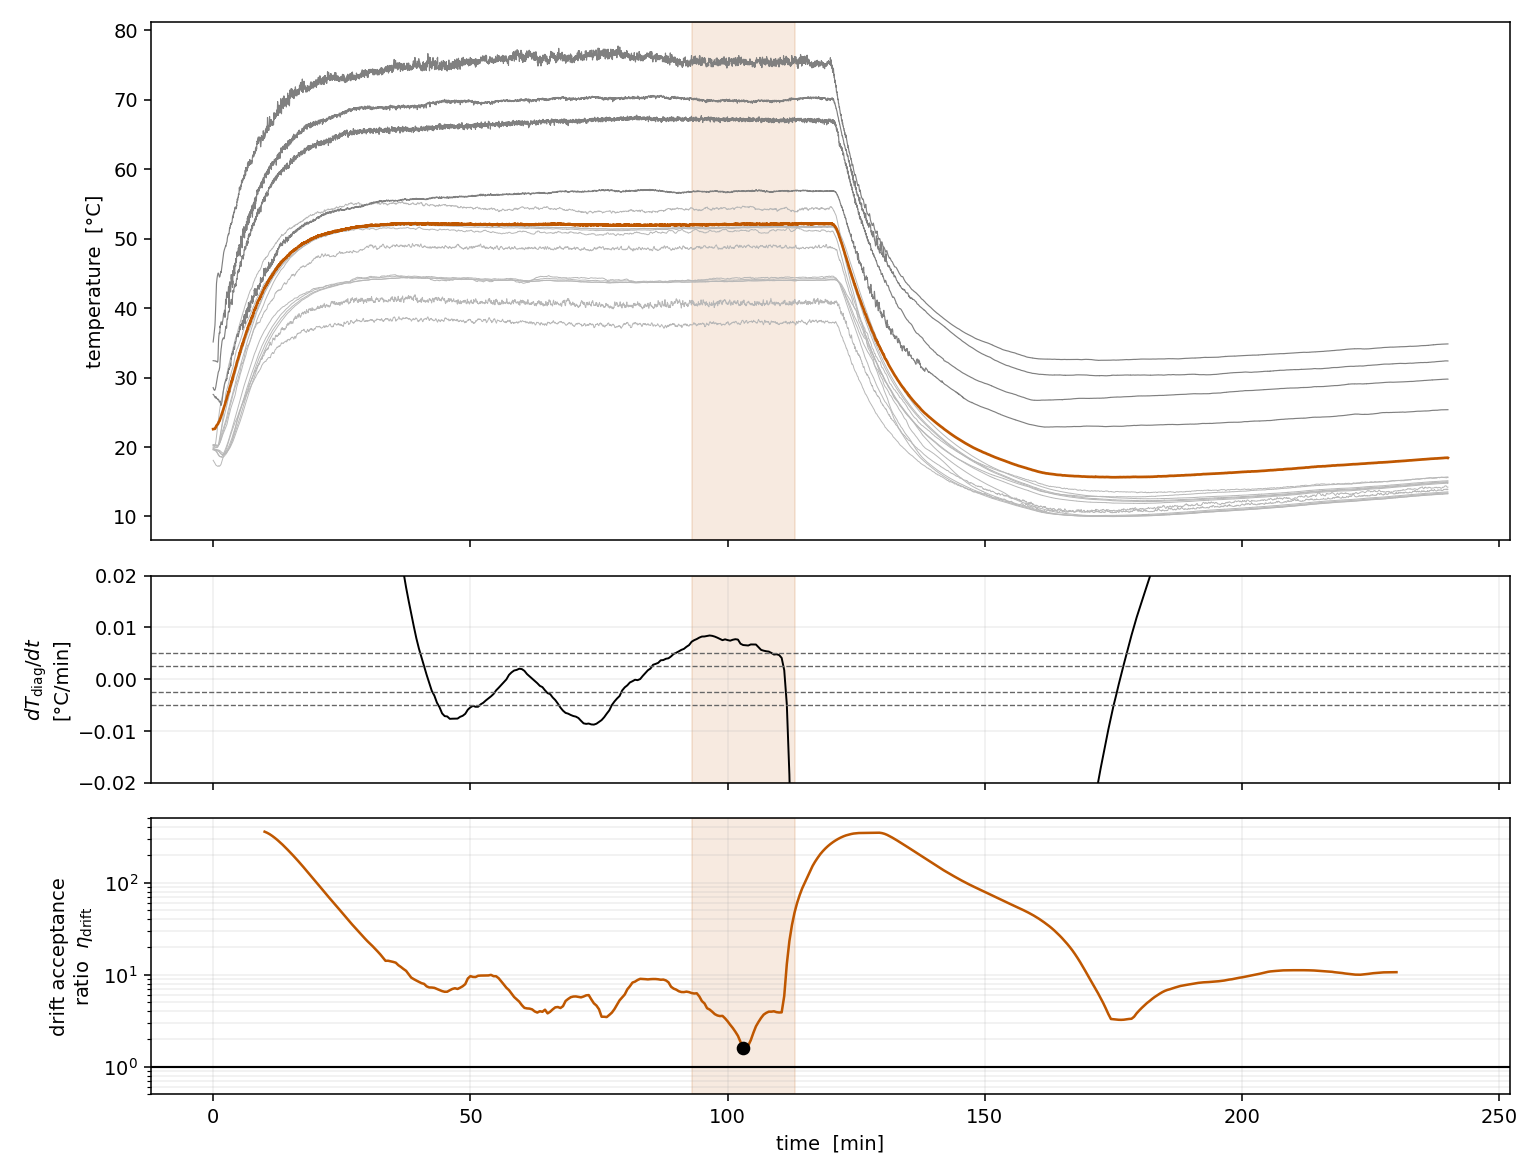
\includegraphics[width=0.90\textwidth]{images/prop30_ss_detection_newmethod.png}
\caption{Operating-class steady-state diagnostic for the example run.
\textbf{Top:} the sixteen loop thermocouples and the diagnostic mean $\Tdiag$.
\textbf{Middle:} centered-window drift of $\Tdiag$ against the operating and
calibration limits. \textbf{Bottom:} $\eta_{\mathrm{drift}}$ on a logarithmic
axis, where passing requires $\eta_{\mathrm{drift}}\leq1$. The shaded
\SIrange{93}{113}{min} window minimizes the ratio at
$\eta_{\mathrm{drift,min}}=\num{1.60}$, limited by $\Tdiag$.}
\label{fig:ss_detection}
\end{figure}

Two plotting conventions in Figure~\ref{fig:ss_detection} are worth noting.
Because the analysis uses centered windows, $\eta_{\mathrm{drift}}$ is
undefined within \SI{10}{min} of either record endpoint. The middle panel is
clipped to $\pm\SI{0.02}{\degreeCelsius\per min}$ so that the acceptance bands
remain visible, and the lower panel is logarithmic so that the pass value of
unity stays distinguishable from the observed minimum.

\textbf{Result.} No interval met the acceptance criteria, so no steady-state
values are reported for this run. Table~\ref{tab:candidate} summarizes the most
favorable window and why it failed: the limiting quantity is the diagnostic
mean, whose $|b|+2u_b=\SI{0.0080}{\degreeCelsius\per min}$ exceeds its
operating limit by a factor of \num{1.60}. The supporting environmental checks
and the independent energy residual were not needed, since neither can reverse
a failed drift criterion.

\begin{table}[H]
\centering
\caption{Best candidate window: rejected diagnostic summary. Reported as a
diagnostic, not as an accepted steady state.}
\label{tab:candidate}
{\small
\renewcommand{\arraystretch}{1.18}
\begin{tabularx}{0.86\textwidth}{@{}>{\raggedright\arraybackslash}X>{\raggedleft\arraybackslash}p{2.5in}@{}}
\toprule
\textbf{Item} & \textbf{Value} \\
\midrule
Candidate start and end time & \SI{93.0}{min} to \SI{113.0}{min} \\
Window center time plotted in Figure~\ref{fig:ss_detection} & \SI{103.0}{min} \\
Evaluation-window length $W_{\mathrm{eval}}$ & \SI{20}{min} \\
Minimum drift acceptance ratio $\eta_{\mathrm{drift}}$ & \num{1.60} \\
Limiting quantity & $\Tdiag$ (diagnostic mean) \\
Limiting slope $b$ & \SI{+0.0066}{\degreeCelsius\per min} \\
HAC contribution $2u_b$ & \SI{0.0014}{\degreeCelsius\per min} \\
Applicable limit $b_{\mathrm{crit}}$ & \SI{0.0050}{\degreeCelsius\per min} \\
Four-point fluid mean $\Tavg$ & \SI{67.32}{\degreeCelsius} \\
Internal-fluid max$-$min spread & \SI{18.62}{\degreeCelsius} \\
Heater duty $\QHs$ & not recorded in this run \\
Cooler duty $\QCs$ & not recorded in this run \\
Final disposition & Rejected \\
\bottomrule
\end{tabularx}}
\end{table}

Leg-referenced quantities such as $\Delta T_{\mathrm{loop}}$ are omitted from
Table~\ref{tab:candidate} because the \texttt{PTC} channels could not be mapped
confidently to loop stations. The four-point mean $\Tavg$ and the internal-fluid
spread are order-independent and remain reportable.

\subsubsection{Time constant}

The rejection above is not merely a threshold outcome; the record also shows
why an operating plateau is the wrong place to measure the loop's thermal time
scale. Across the nominal high-temperature plateau the diagnostic-mean drift
decays as the loop equilibrates, but fitting an exponential to it, in either
the derivative domain ($|d\Tdiag/dt|$) or the temperature domain ($\Tdiag$
itself), returns a time constant that varies by more than an order of magnitude
with the chosen fit interval. The residual approach to equilibrium is small and
confounded with the wander described below, so the fit is not identifiable.
This is the case cited in \PhaseTwoDoc, Section~2, ``Slowest loop time constant, and no plateau-derived
time constant is reported here.

The same record contains a contrasting case. Near \SI{129}{min} the
temperatures fall system-wide in a manner consistent with a shutdown, giving an
unforced relaxation transient. Fitting the diagnostic mean over the monotonic
interval $I_c\approx[\SI{129}{min},\SI{165}{min}]$, which ends before later
reheating becomes material, to
\begin{equation}
\Tdiag(t)=T_{\infty,\mathrm{eff}}
+\Delta T\exp\!\left[-\frac{t-t_{c,0}}{\tau_{\mathrm{eff,cool}}}\right]
\label{eq:prelim_cooldown_fit}
\end{equation}
gives $\tau_{\mathrm{eff,cool}}\approx\SI{15}{min}$ with a fit-start
sensitivity of \SIrange{13}{17}{min}, $R^2>0.999$, and
$T_{\infty,\mathrm{eff}}\approx\SI{15}{\degreeCelsius}$
(Figure~\ref{fig:a1}(b)). The point of the comparison is methodological: a
genuine relaxation transient, even an uncontrolled one, determines a time
constant that the plateau cannot, which is why
\PhaseTwoDoc, Section~2, ``Slowest loop time constant requires $\tau_{\mathrm{slow}}$ to come from the
Phase~2 relaxation tests.

That said, this fit is preliminary in three respects. The archived record does
not identify whether the heater alone or both heater and cooler were shut down,
nor the secondary-flow states. The result is a property of the unweighted
diagnostic mean over one interval: it is neither $\tau_{\mathrm{slow}}$ nor a
full-facility $C/UA$ time constant, and the fitted asymptote is not
demonstrated to equal the measured room temperature. The
\SIrange{13}{17}{min} span is a fit-window sensitivity, not a confidence
interval. It shall not be used to set a campaign hold time.

\subsubsection{Residual wander}

Over the nominal plateau-analysis interval
$I_w=[\SI{50}{min},\SI{118}{min}]$ the diagnostic temperature fluctuates by a
few tenths of a degree Celsius about its local trend. The trace changes
behavior near \SI{68}{min}, but no contemporaneous control, secondary-flow, or
data-system event record is available, so the interval is preliminary and shall
not be treated as a confirmed homogeneous segment. In the formal campaign, an
analysis interval shall be split at every logged event and each segment
evaluated separately.

To quantify the fluctuation without mixing temperature and temperature-rate
units, detrend the diagnostic temperature over $I_w$ with a low-order trend,
\begin{equation}
T_{\mathrm{diag,fit}}(t)=T_0+c_T\,(t-t_0),
\qquad
r_T(t)=\Tdiag(t)-T_{\mathrm{diag,fit}}(t),
\label{eq:wander_trend}
\end{equation}
then form non-overlapping \SI{30}{s} block averages $\overline r_{T,k}$, the
same blocks used by the detector, and report
\begin{equation}
A_{\mathrm{wander,pp}}=\max_k\overline r_{T,k}-\min_k\overline r_{T,k},
\qquad
A_{\mathrm{wander,90}}=Q_{0.95}(\overline r_T)-Q_{0.05}(\overline r_T).
\label{eq:wander_amplitude}
\end{equation}
The first is a block-averaged peak-to-peak range, the second a more
spike-resistant central-\SI{90}{\percent} range. Figure~\ref{fig:a1}(a) shows
the unsmoothed residual, whose raw peak-to-peak span is about
\SI{0.3}{\degreeCelsius}; the estimate is insensitive to the choice of
low-order detrend, though a raw maximum-minus-minimum is not robust to isolated
samples.

This motion matches the wander defined in Section~\ref{sec:steady_criteria},
but the temperature record alone cannot separate it from secondary-control
cycling, room-temperature forcing, or another thermal mode. Its dominant
timescale is not cleanly periodic and is comparable to the evaluation window,
so a window can land near a turning point and return a momentarily small slope
that is not evidence of steadiness. Because the motion is not periodic, it also
does not qualify for the statistically stationary case of
Section~\ref{sec:stationary_state}.

\begin{figure}[H]
\centering
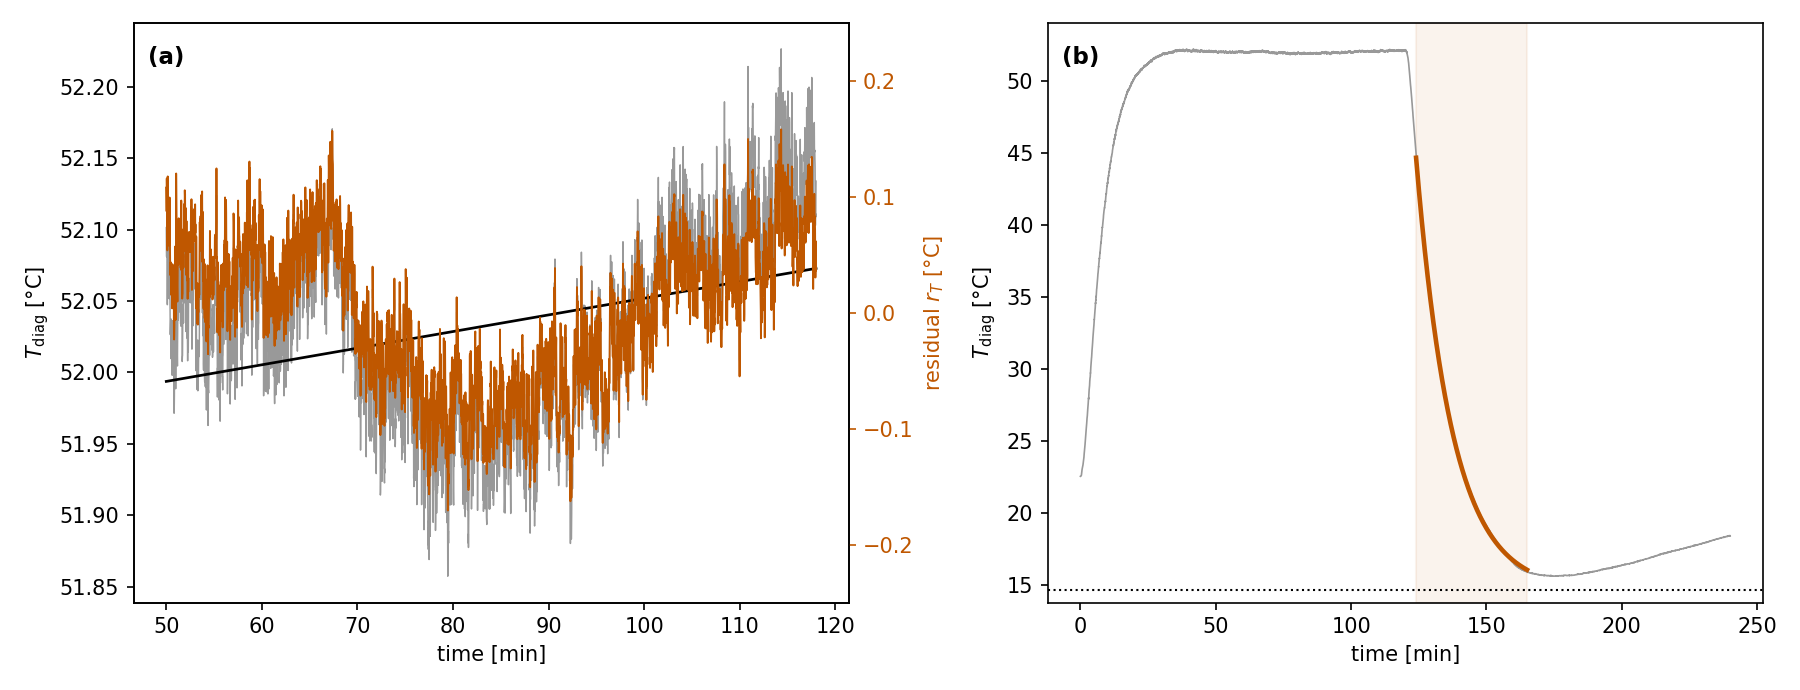
\includegraphics[width=0.98\textwidth]{images/A1_figure.png}
\caption{Preliminary diagnostics for the archived run. \textbf{(a)} Wander over
$I_w$: the diagnostic mean $\Tdiag$ (gray, left axis), its linear detrend
(black), and the unsmoothed residual $r_T$ (orange, right axis).
\textbf{(b)} Shutdown relaxation: the fit of
Equation~\eqref{eq:prelim_cooldown_fit} over the shaded interval $I_c$, with
the fitted asymptote $T_{\infty,\mathrm{eff}}$ shown dotted.}
\label{fig:a1}
\end{figure}

Taken together, the two features bound what this record can support. Across
portions of the plateau the centered-window diagnostic-mean drift stays near
\SIrange{0.005}{0.010}{\degreeCelsius\per min}, at or above the
calibration-quality limit, and the record cannot distinguish an unfinished soak,
which a longer hold would cure, from persistent wander, which it would not.
Whether the tabulated limits are reachable on this facility is therefore not
established here. What the record does establish is that this run is not steady
to operating tolerance, and that the acceptance method identifies the limiting
signal and quantifies the shortfall rather than returning a bare pass or fail.

\clearpage
\addcontentsline{toc}{section}{References}
{\small
\begin{thebibliography}{9}
\setlength{\itemsep}{1.5pt}
\setlength{\parskip}{0pt}

\bibitem{jcgm100}
Joint Committee for Guides in Metrology, \emph{Evaluation of Measurement Data---Guide to the Expression of Uncertainty in Measurement}, JCGM~100:2008, 2008. \href{https://doi.org/10.59161/JCGM100-2008E}{doi:10.59161/JCGM100-2008E}.

\bibitem{neweywest1987}
W. K. Newey and K. D. West, ``A simple, positive semi-definite, heteroskedasticity and autocorrelation consistent covariance matrix,'' \emph{Econometrica}, vol.~55, no.~3, pp.~703--708, 1987. \href{https://doi.org/10.2307/1913610}{doi:10.2307/1913610}.

\bibitem{cao1995}
S. Cao and R. R. Rhinehart, ``An efficient method for on-line identification of steady state,'' \emph{Journal of Process Control}, vol.~5, no.~6, pp.~363--374, 1995. \href{https://doi.org/10.1016/0959-1524(95)00009-F}{doi:10.1016/0959-1524(95)00009-F}.

\bibitem{cao1997}
S. Cao and R. R. Rhinehart, ``Critical values for a steady-state identifier,'' \emph{Journal of Process Control}, vol.~7, no.~2, pp.~149--152, 1997. \href{https://doi.org/10.1016/S0959-1524(96)00026-1}{doi:10.1016/S0959-1524(96)00026-1}.

\end{thebibliography}
}




\clearpage
\appendix
\section{Nomenclature}
\label{sec:nomenclature}
A dot denotes a rate, a hat denotes an estimate or model prediction, an overbar denotes an interval or block mean as stated in context, and $u_x$ denotes the standard uncertainty of quantity $x$. Only symbols used in this phase document are included below.

\begingroup
\footnotesize
\setlength{\LTpre}{4pt}
\setlength{\LTpost}{10pt}
\setlength{\tabcolsep}{4pt}
\renewcommand{\arraystretch}{1.10}
\begin{longtable}{@{}>{\raggedright\arraybackslash}p{1.78in}>{\raggedright\arraybackslash}p{1.08in}>{\raggedright\arraybackslash}p{3.62in}@{}}
\caption{Phase 1 nomenclature.}\label{tab:nomenclature}\\
\toprule
\textbf{Symbol} & \textbf{Units} & \textbf{Description} \\
\midrule
\endfirsthead
\multicolumn{3}{l}{\small\itshape Table~\ref{tab:nomenclature} continued from previous page}\\
\toprule
\textbf{Symbol} & \textbf{Units} & \textbf{Description} \\
\midrule
\endhead
\bottomrule
\endfoot
$T$ & \si{\degreeCelsius} & Generic measured temperature. \\
$T_{H,in},T_{H,out},T_{C,in},T_{C,out}$ & \si{\degreeCelsius} & Primary temperatures at the heater and cooler measurement planes. \\
$T_j,\,T_{w,i}$ & \si{\degreeCelsius} & Generic internal-fluid and under-insulation wall temperatures. \\
$\Tamb,\,T_{\mathrm{amb},i}$ & \si{\degreeCelsius} & Representative and region-specific room-air temperatures. \\
$\Thot,\,\Tcold,\,\Tavg,\,\Delta T_{\mathrm{loop}}$ & \si{\degreeCelsius} & Hot-leg, cold-leg, four-point mean, and loop temperature-difference coordinates. \\
$\Delta T_{\mathrm{spread}},\,\Delta T_{w,\mathrm{spread}},\,\Delta T_{f-w}$ & \si{\degreeCelsius} & Four-point fluid spread, wall-profile spread, and internal--wall mean offset. \\
$\Delta T_{\mathrm{iso,eng}}$ & \si{\degreeCelsius} & Near-isothermal engineering limit. \\
$\Tdiag$ & \si{\degreeCelsius} & Unweighted sixteen-channel structural-storage diagnostic mean. \\
$\Delta T_H,\,\Delta T_C$ & \si{\degreeCelsius} & Signed primary temperature changes across the heater and cooler. \\
$\mathbf J,\,\boldsymbol\Sigma_x$ & Mixed & Sensitivity row vector and covariance matrix in uncertainty propagation. \\
$x_i,\,x_{i,k},\,\hat x_i$ & Signal units & Input quantity, observation, and reported interval mean. \\
$a_i,\,b_i,\,b_{\mathrm{crit},i},\,u_b$ & Mixed & Intercept, fitted slope, slope-equivalence limit, and slope uncertainty. \\
$W_{\mathrm{eval}},\,W_{\mathrm{rep}},\,W_{\mathrm{hold}}$ & \si{\minute} & Evaluation, reporting, and continuous-acceptance hold durations. \\
$\eta_{\mathrm{drift}},\,\rho_i$ & -- & Worst normalized trend ratio and per-signal trend margin ratio. \\
$N,\,N_{\mathrm{eff},i},\,M,\,M_{\min}$ & -- & Raw/effective sample counts and numbers of independent blocks. \\
$\Delta t,\,L_i,\,\widehat\rho_i(\ell),\,\tau_{\mathrm{int},i}$ & Mixed & Sample interval, retained lag, autocorrelation, and integrated autocorrelation time. \\
$u_x,\,u_A(x),\,\gamma_{\Delta T},\,\gamma_{\mathrm{res}}$ & Mixed & Combined/Type-A uncertainties and project resolution allocations. \\
$\QHs,\,\QCs$ & \si{\watt} & Heater duty supplied and cooler duty removed on the secondary side. \\
$\dot Q_{a,H},\,\dot Q_{a,C}$ & \si{\watt} & Ambient losses from the heater and cooler control volumes. \\
$h(T,c),\,\Delta h_H,\,\Delta h_C$ & \si{\joule\per\kilogram} & Specific enthalpy and signed primary exchanger enthalpy changes. \\
$\mdotp,\,\mdotpH,\,\mdotpC,\,\hat{\mdotp}$ & \si{\kilogram\per\second} & Signed primary flow, exchanger estimates, and reconciled estimate. \\
$\lambda_m,\,\tau_m,\,\tau_{\mathrm{slow}},\,\tau_{\mathrm{slow,op}}$ & Mixed & State-matrix eigenvalue, modal time constant, slowest time constant, and conservative operational settling value. \\
$i,j,k,m,\ell,\mathcal N_i,c$ & -- & Measurement/model indices, coupled-region set, and documented fluid composition. \\
\end{longtable}
\endgroup

\end{document}
